\section{Hardwareimplementering}
<<<<<<< HEAD
Alle dele af projektets hardware er blevet analyseret og designet og derefter implementeret. Vi startede med at udregne komponenter til forstærkeren, som vi på forhånd vidste hvordan skulle opbygges. Efter beregningerne kunne forstærkeren opbygges på fumlebræt. Efter at hver del er blevet implementeret på fumlebrættet er det blevet modultestet. På denne måde er vi sikre på, at hvert delelement af projektets hardware virker som forventet. På fumlebrættet er forstærkeren, subtractoren og Sallen-Key filteret derved implementeret og modultestet enkeltvis for at se om de gav de forventede værdier. Efterfølgende blev det hele sat sammen til et kredsløb og systemet kunne derefter integrationstestes. 

\begin{figure}[h!]
	\centering
	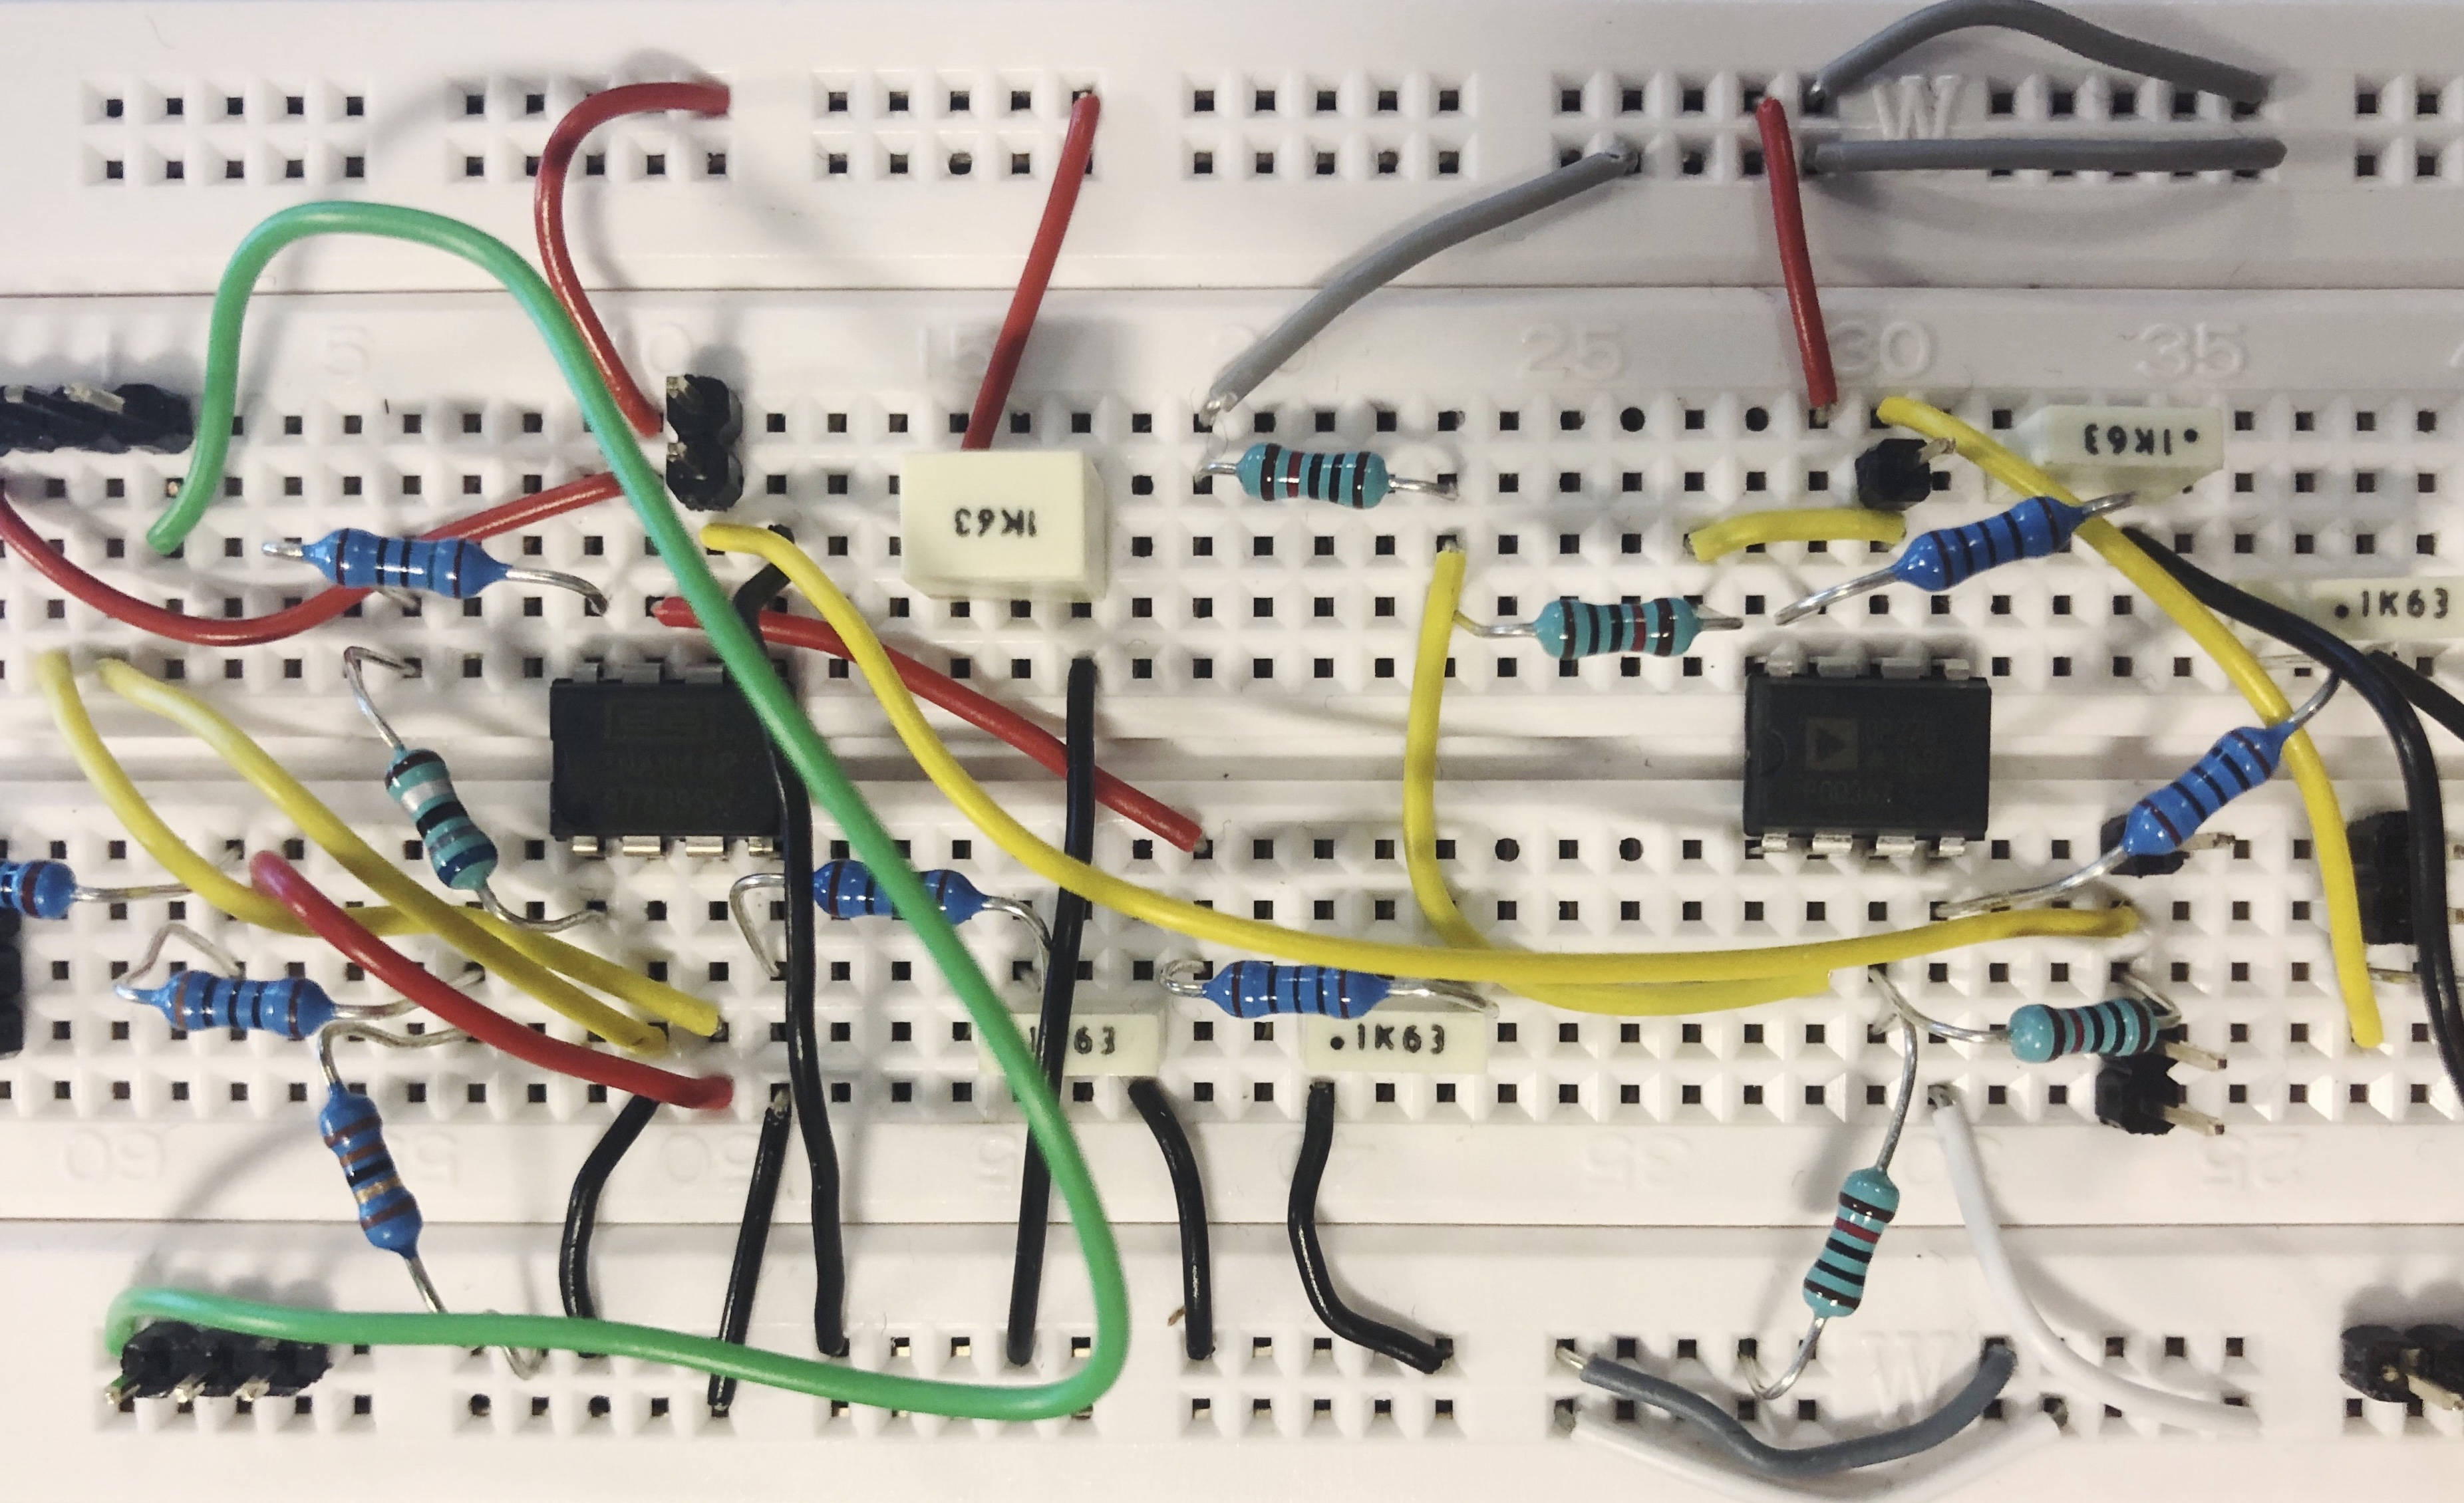
\includegraphics
	[width=0.54\linewidth]{../Rapport/Implementering_og_test/Hardware/forstaerkerogsubtractor2}
	\caption{Opbygning af forstærker(til venstre) og subtractor (til højre) på fumlebræt}
	\label{fig:forstaerkerogsubtractor1}
\end{figure}

\begin{figure}[h!]
	\centering
	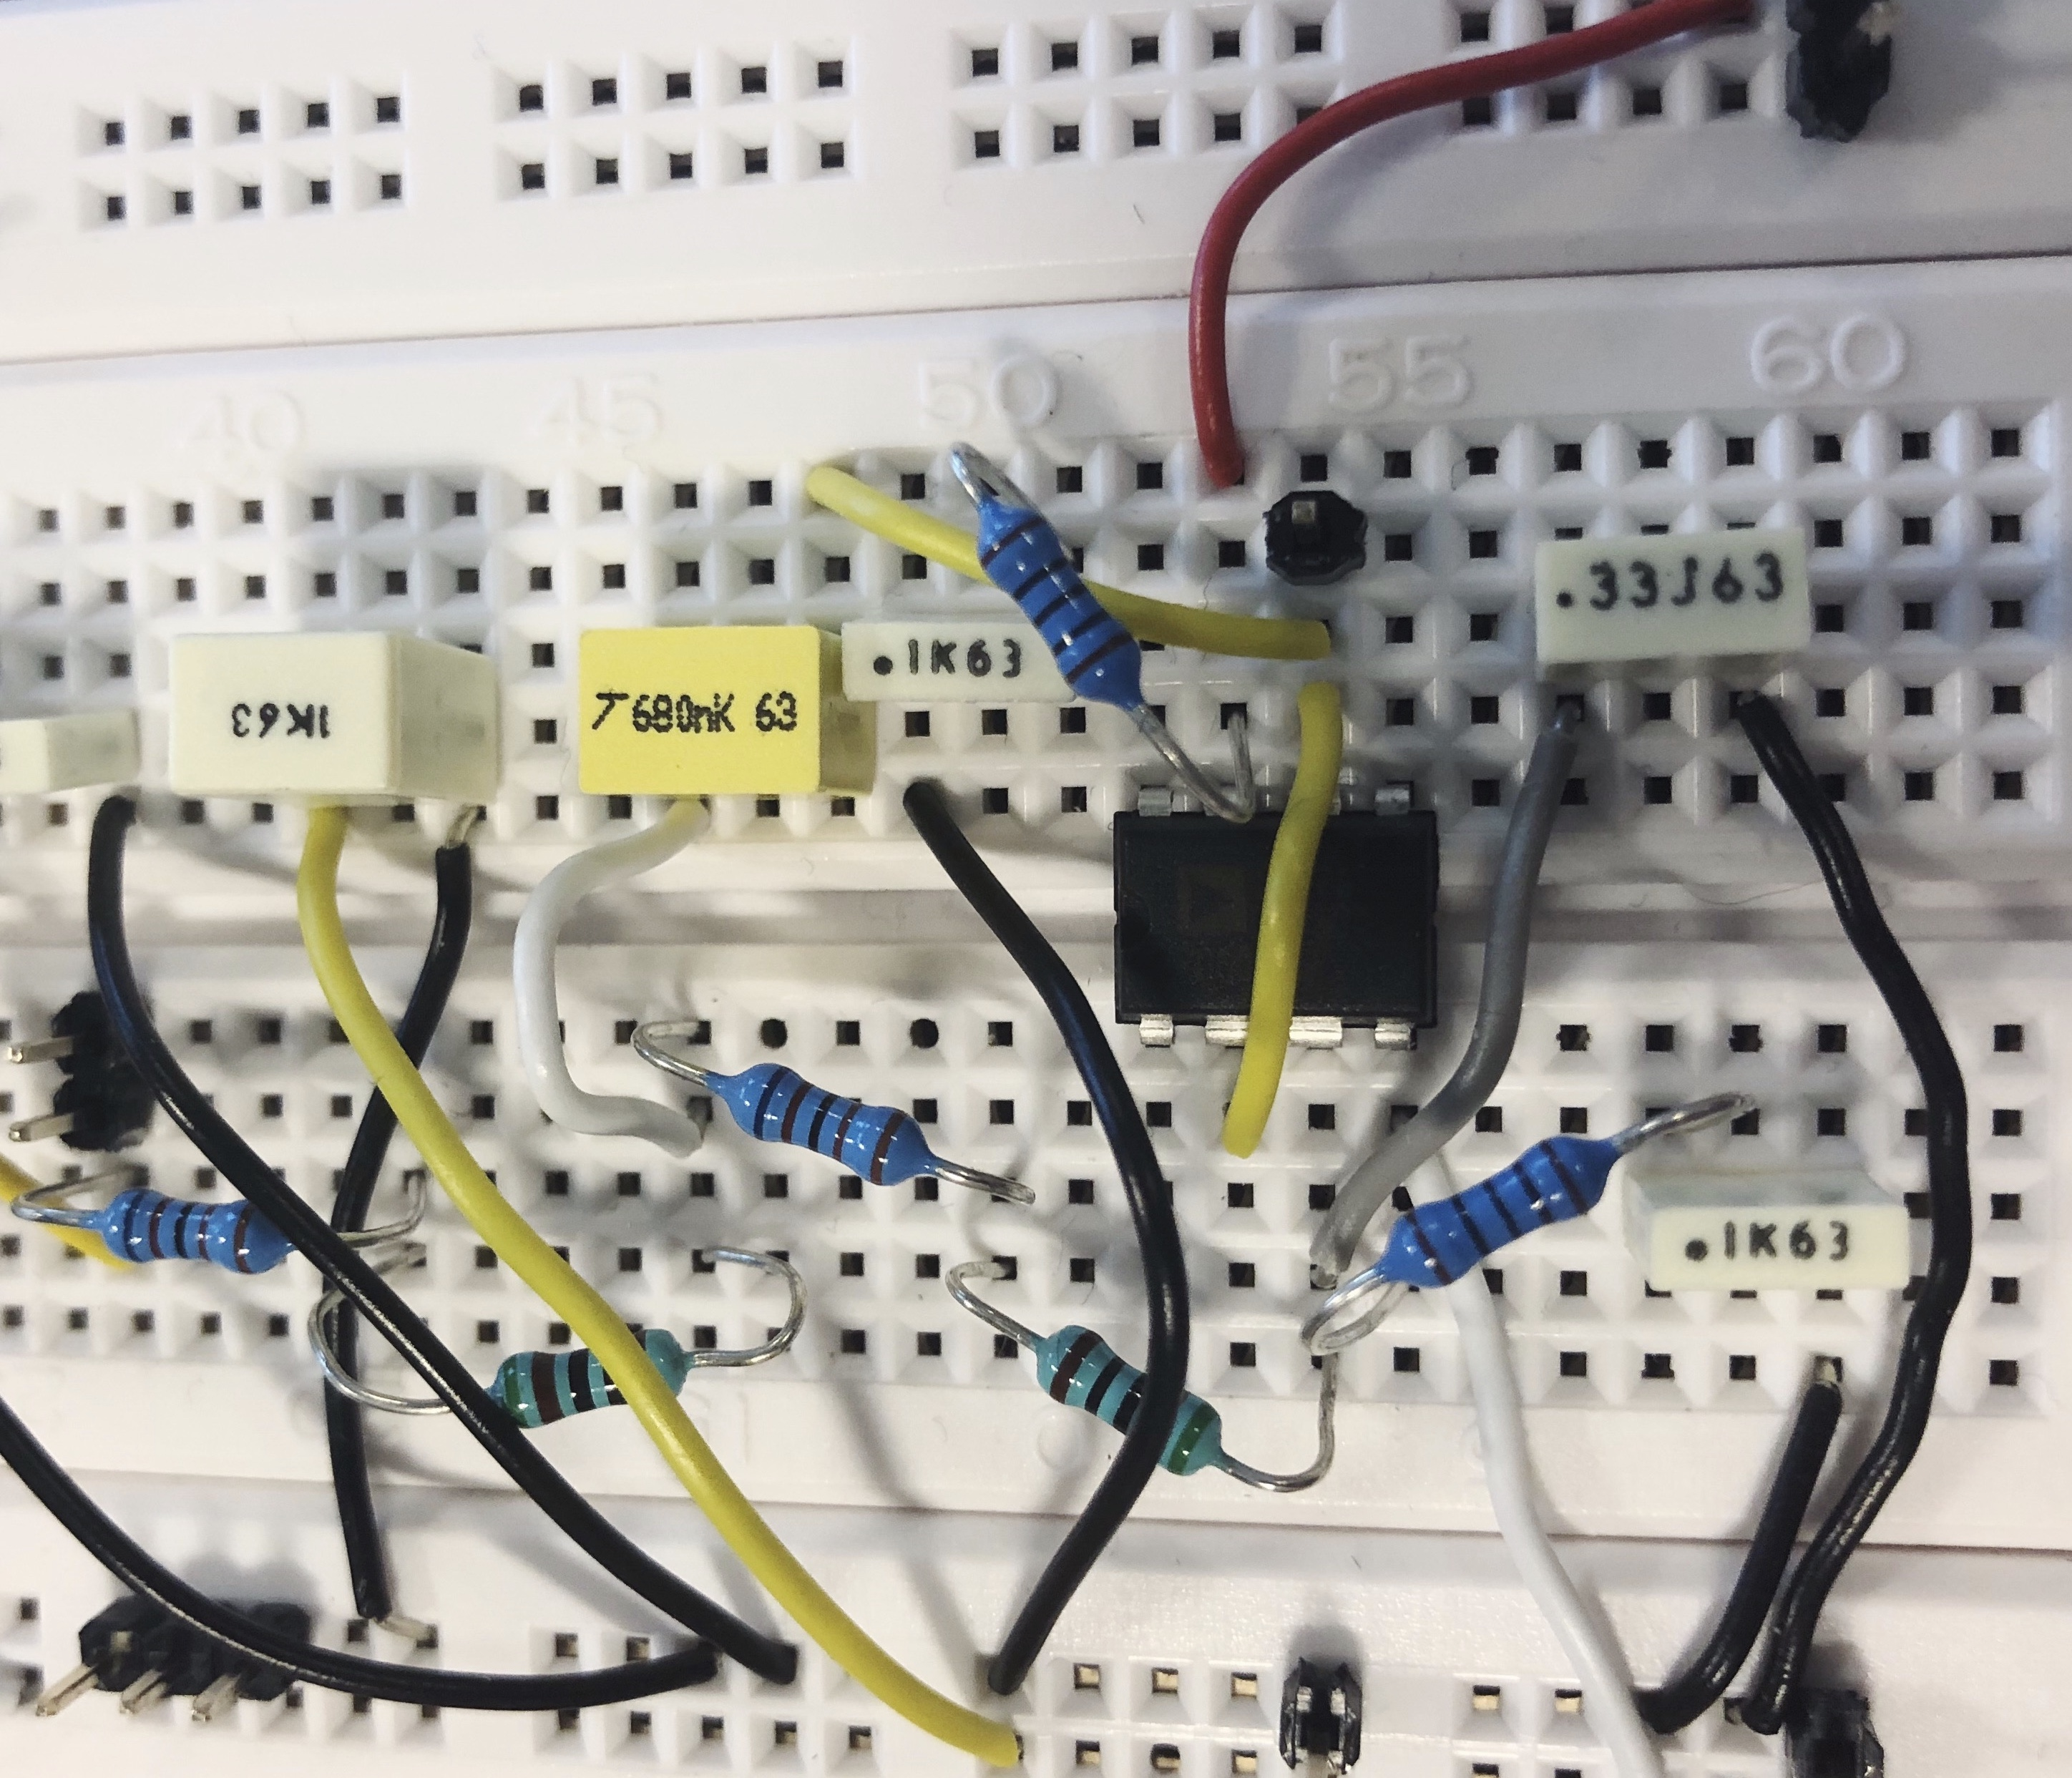
\includegraphics
	[width=0.54\linewidth]{../Rapport/Implementering_og_test/Hardware/filter2}
	\caption{Opbygning af filter på fumlebræt}
	\label{fig:filter1}
\end{figure}

Efter integrationstesten blev kredsløbet tegnet i Multisim. Det tegnede kredsløb i Multisim blev til slut overført til ultiboard, hvor de tilhørende komponenter blev placeret på printpladen. Printet blev testet og sendt til EuroCircuits. De beregnede komponenter i analyse-delen er til slut loddet på den færdige printplade og systemet blev testet en sidste gang. 

For kredsløbet i Multisim henvises til figur \vref{fig:Multisim2}. Nedenfor vises designet af printpladen i Ultiboard da det var klar til print samt printpladen, der er loddet med alle komponenter.

\begin{figure}[h!]
	\centering
	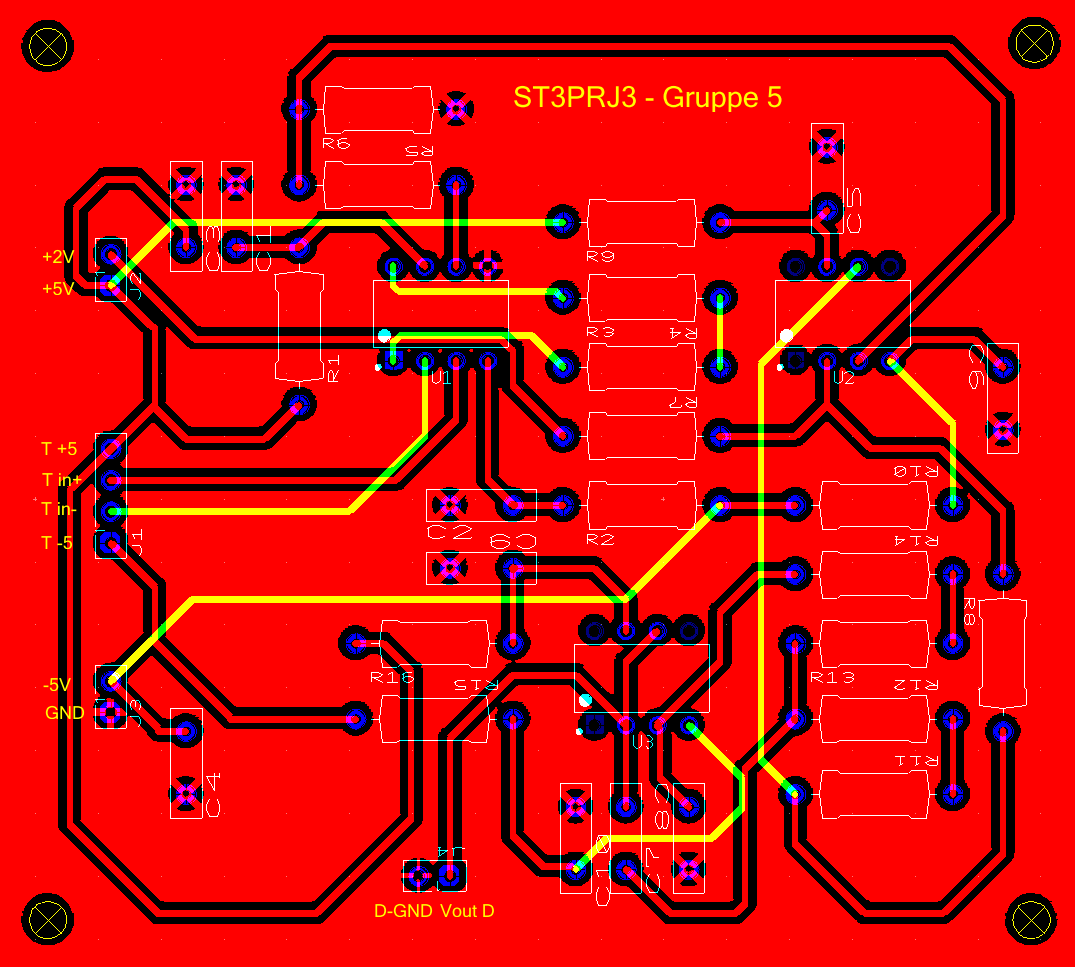
\includegraphics[width=0.5\linewidth]{../Rapport/Implementering_og_test/Hardware/Ultiboard}
	\caption[Print i Ultiboard]{}
	\label{fig:ultiboard1}
\end{figure}

=======
Hardware er implementeret således at den indeholder en PC, NI DAQ 6009( AD-converter), Sallen-Key Lavpas-filter, transducer og substraktor. På fumlebrættet er selve forstærkeren, filteret og substraktoren opbygget. Disse tre dele er hver især blevet testet igennem, for at se om de gav de forventede værdier. Det hele blev sat sammen til et kredsløb og der blev testet for hele systemet. Dette blev gjort for at sikre, at systemet i helhel virkede som der blev forventet. Efter testningen af hele systemet, blev kredsløbet lavet inde på multisim, hvor multisimkredsløbet derefter blev overført til ultiboard, hvor de tilhørende komponenter blev placeret og sat fast på printpladen.  Printet blev derefter sendt til afsted og vi fik vores printplade. Herefter loddede vi på egen hånd de udregnede komponenter. 

BILLEDE AF PRINTET OG ULTIBOARD

Systemet hænger sammen på den måde, at strømforsyningen forsyner med strøm til substraktoren, transduceren,  og forstærkeren. Analog discovery forsyner spænding til forstærker, transducer og filter.
Signalet, som i form af et blodtrykssignal, kommer fra transduceren til Analog Discovery.  Forstærkeren forstærker signalet fra transduceren, der sender signalet gennem filteret, som bliver filtreret. Signalet går igennem substraktoren, som neddæmper signalet til at gå fra 0-4 V til +- 2 V . Dette signal bliver sendt videre til DAQ’en, som omdanner det analoge signal til et digitalt signal, der sender signalet videre til PC’en. 
>>>>>>> 9656cb1b8b2eb4bcac12ea1597f7c5a821fee169



\section{Test af hardware}
\subsection{Forstærker}

\subsubsection{Test med Analog Discovery}
\subsubsection{Test med væskesøjle}
\subsection{Anti-aliaseringsfilter}
\subsubsection{Test med Analog Discovery}
\subsubsection{Test med væskesøjle}
\subsection{Test af printplade}
